\documentclass[
	a4paper, % Paper size, use either a4paper or letterpaper
	12pt, % Default font size, the template is designed to look good at 12pt so it's best not to change this
	%unnumberedsections, % Uncomment for no section numbering
]{article}
\usepackage[a4paper,top=0.4cm, bottom=0.8cm, left=1.6cm, right=1.6cm]{geometry}

\usepackage{cmap} % make PDF files searchable and copy-able
\usepackage[utf8]{inputenc}
\usepackage[english,russian]{babel}

\usepackage{amssymb,amsmath}
\renewcommand {\phi}{\varphi}
\usepackage{mathtext}

\usepackage{libertine}
\usepackage[libertine]{newtxmath}

\usepackage{graphicx} % Required for inserting images
\graphicspath{{./img/}} % Destination of images
\usepackage{subcaption}

\usepackage{hyperref}

\usepackage{xcolor}



% opening
\title{
	\textcolor{cyan}{Отчет о выполнении лабораторной работы 1.2.1}
	\\
	Определение скорости полета пули при помощи баллистического маятника
}
\author{Шубин Владислав, Байбулатов Амир}
%\date{Сентябрь 2023}

\begin{document}    
	
	\maketitle
	
	\section{Аннотация}
	В работе определяется скорость полета пули, путём применения законов сохранения и использования баллистического маятника. Используется следующий метод измерений скорости: 1) определение отклонения маятника с помощью оптической системы, изображенной на рис. \ref{fig:subim1} Длины нитей измеряются с помощью сантиметровой линейки, отклонения маятника с помощью миллиметровой линейки. Детально исследуется систематические и случайные погрешности проводимых измерений.
	
	
	\section{Теоретические сведения}
	
	\subsection{Метод баллистического маятника, совершающего поступательное движение}
	
	В этой части работы (вторая часть не выполнялась) используется установка, изображенная на рис. \ref{fig:subim1}. Внешними силами для системы пуля-цилиндр являются сила тяжести, не имеющая горизонтальной компоненты, и силы натяжения нитей, горизонтальные компоненты которых появляются при отклонении маятника. Но так как отклонения маятника малы, то и эти компоненты малы и тем более мал и их импульс. Поэтому закон сохранения импульса при соударении пули с цилиндром имеет вид
	\begin{equation}
		mu = (M + m)V.
	\end{equation}
	Здесь m - масса пули, M - масса цилиндра, V - скорость цилиндра и пули после неупругого соударения.
	
	Откуда (учитывая, что M >> m) можно написать
	\begin{equation}
		u = \frac{M}{m}V.
	\end{equation}
	
	По закону сохранения энергии
	
	\begin{equation}
		V^2 = 2gh.
	\end{equation}
	Здесь g - ускорение свободного падения, h - высота подъёма маятника над его начальным положением.
	
	Высота подъёма маятника выражается через угол $\phi$ отклонения маятника от вертикали:
	\begin{equation}
		h = L(1 - \cos{\phi}) = 2L\sin^2{\frac{\phi}{2}},
	\end{equation}
	где $\phi$ $\approx$ $\frac{\Delta x}{L}$
	
	Из (2), (3) и (4) получаем формулу для определения скорости пули:
	\begin{equation}
		v = \frac{M}{m}\sqrt{\frac{g}{L}}\Delta x.
	\end{equation}
	
	
	\begin{figure}[h]
		
		\begin{subfigure}{0.5\textwidth}
			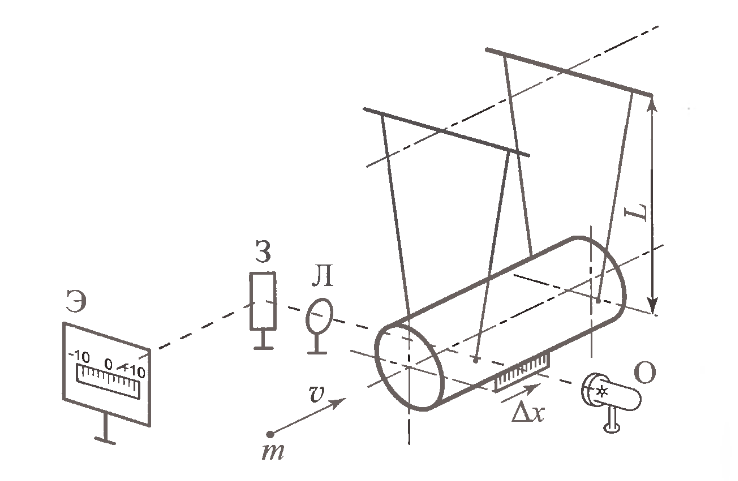
\includegraphics[width=0.9\linewidth]{1.png} 
			\caption{Рис. 1. Схема установки для измерения\\ скорости полета пули}
			\label{fig:subim1}
		\end{subfigure}
		\begin{subfigure}{0.5\textwidth}
			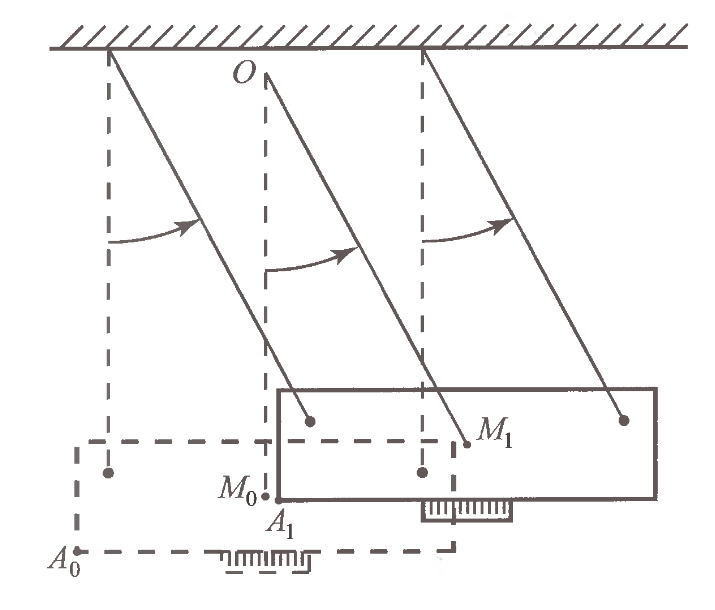
\includegraphics[width=0.9\linewidth]{2.png}
			\caption{Рис 2. Поведение баллистического маятника\\ при попадании в него пули}
			\label{fig:subim2}
		\end{subfigure}
		
	\end{figure}
	
	\section{Оборудование и инструментальные погрешности}
	\textbf{Оборудование:} духовое ружье на штативе, осветитель, оптическая система для измерения отклонений маятника, измерительная линейка, пули и весы для их взвешивания, а также баллистические маятники.
	\begin{itemize}
		\item \textbf{Оптическая система}: $\Delta \text{сис} = \pm0.25$ мм (по цене деления)
		\item \textbf{Линейка}: $\Delta \text{лин} = \pm1$ см (по цене деления)
		\item \textbf{Весы}: $\Delta m = \pm{5}$ мг (маркировка производителя)
	\end{itemize}
	
	%\newpage
	
	\section{Результаты измерений и обработка данных}
	
	\subsection{Характеристики системы:}
	
	$L = 2,22\pm 0,01$ м,\\
	$M=2905\pm5$ г.
	
	\subsection{Измерения:}
	
	\begin{table}[h]
		\centering
		\begin{tabular}{|c|c|c|c|c|c|c|c|c|c|c|}
			\hline
			N изм. & 1 & 2 & 3 & 4 & 5 & 6 & 7 & 8 & 9 & 10  \\
			\hline
			m, г & 0.516 & 0.515 & 0.503 & 0.504 & 0.507 & 0.512 & 0.508 & 0.507 & 0.509 & 0.501 \\
			\hline
		\end{tabular}
		\caption{Результаты измерений масс пулек.}
		\label{table:1}
	\end{table}
	
	%\newpage
	
	\begin{table}[h]
		\centering
		\begin{tabular}[H]{|c|c|c|c|c|c|c|c|c|c|c|}
			\hline
			$x_0$, мм & -0.8 & 0.0 & 0.5 & 1.0 & -1.5 & -1.8 & -1.5 & -1.0 & -0.5 & -0.3  \\
			\hline
			$x_1$, мм & 12.0 & 11.6 & 12.5 & 12.5 & 10.5 & 10.5 & 10.3 & 10.2 & 10.6 & 11.9  \\
			\hline
			$x_2$, мм & 11.7 & 11.4 & 12.3 & 12.4 & 10.4 & 10.4 & 10.2 & 10.1 & 10.5 & 11.7  \\
			\hline
			$x_3$, мм & 11.5 & 11.4 & 12.2 & 12.3 & 10.3 & 10.3 & 10.0 & 10.0 & 10.4 & 11.6  \\
			\hline
			$x_{\text{ср}}$, мм & 11.7 & 11.5 & 12.3 & 12.4 & 10.4 & 10.4 & 10.2 & 10.1 & 10.5 & 11.7  \\
			\hline
		\end{tabular}
		\caption{Результаты измерений отклонений маятника.}
		\label{table:2}
	\end{table}
	\begin{table}[h]
		\centering
		\begin{tabular}[H]{|c|c|c|c|c|c|c|c|c|c|c|}
			\hline
			$\Delta x_{\text{ср}}$, мм & 12.5 & 11.5 & 11.8 & 11.4 & 11.9 & 12.2 & 11.7 & 11.1 & 11.0 & 12.0  \\
			\hline
			$u$, м/c & 148.0 & 136.4 & 143.3 & 138.2 & 143.4  & 145.5 & 140.7 & 133.7 & 132.0 & 146.3  \\
			\hline
		\end{tabular}
		\caption{Результаты вычислений скорости пули.}
		\label{table:3}
	\end{table}
	
	\newpage
	
	Рассчитаем систематическую и случайную погрешности:
	\begin{equation}
		\sigma_u^{\text{сист}} =u \sqrt{\varepsilon_M^2 + \varepsilon_m^2 + \varepsilon_{\Delta x}^2 + \left(\frac{\varepsilon_L}{2} \right)^2}  \;\;\;\;\; \sigma_u^{\text{случ}} = \sqrt{ \frac{1}{n(n-1)} \sum_{i=1}^{n}(u_i - u_{\text{ср}})^2} \;\;\;\;\; \sigma_u =\sqrt{\sigma_{\text{сист}}^2 + \sigma_\text{случ}^2} 
	\end{equation}
	\begin{equation}
		\sigma_u^\text{сист}\approx 3,8 \text{ }\dfrac{\text{м}}{\text{с}} \;\;\;\;\;\;\;\;\;\;\;\;\;\;\;\;\;\;\;\;\;\;\;\;\;\;\;\;\;\;\; \sigma_u^\text{случ}\approx 1,7 \text{ }\dfrac{\text{м}}{\text{с}} \;\;\;\;\;\;\;\;\;\;\;\;\;\;\;\;\;\;\;\;\;\;\;\;\;\;\;\;\;\;\;
\sigma_u \approx 4,2 \text{ }\dfrac{\text{м}}{\text{с}}
	\end{equation}
	
	Тогда средняя скорость $u_\text{ср} = 141,0 \pm 4,2\text{ }\frac{\text{м}}{\text{с}} $
	
	\section{Заключение}
	В работе получено значение скорости пули $u\approx 141,0 \pm 4,2\text{ }\frac{\text{м}}{\text{с}}$. Реальная скорость вылета пули из духового ружья находится в диапазоне 140-200 м/c. Измеренные значения $u$ попали в этот диапазон. Использованный в работе метод баллистического маятника позволил получить значения $u$ образцов с хорошей точностью ({3}\%, состоящей из системных погрешностей величин $M, m, \Delta x, L$, а также случайной погрешности измерений $u$ и $\Delta x$), которая ограничивалась  погрешностями оптической системы, весов и линейки, пренебрежением массой пули в формуле (5), горизонтальными компонентами сил натяжения нитей, а также использованием значения угла в качестве результата функции $\sin$ в связи с его малым значением.
	
	
\end{document}
